\chapter{Literature Review} 
\label{chap:litrev}

This chapter presents the analysis and review of relevant literature conducted throughout this project. The research comprises of literature surrounding different routing algorithms and their current usage within current route planner applications. It also explores other relevant technologies which will be utilised in developing the artefact, such as web frameworks and programming languages.

\section{Background}
\label{litrev:background}
This project has a high level of complexity. It utilises custom, user and system inputs
into a data-driven route planning algorithm, displaying the output on an OpenStreetMap-based web application. 

This review begins with researching literature on different web technologies and programming languages to develop an understanding of what technologies were available to build the proposed system \see{litrev:javascript}\see{litrev:golang}. Once an understanding of the technologies was developed, a review of current competing products was reviewed. This allowed for gaps in the current market to be identified, therefore developing an idea of requirements for the proposed system \see{litrev:competingproducts}. 

Furthermore, research into how cyclists consider different risk factors when planning a ride was key in understanding what routing algorithm was implemented to fit the project's requirements best. An in-depth review of existing literature was conducted to understand two primary risk factors for cyclists: cycling infrastructure \see{litrev:cyclinginfrastructure} and weather conditions \see{litrev:weatherconditions}. 

\section{Research Methods}
\label{litrev:researchmethod}

An initial exploration of sources and subject areas was conducted using Google Chrome to comprehensively understand the topic at hand. Certain regions of interest were also highlighted through crowd-sourcing ideas from knowledgeable individuals. After these areas were outlined, in-depth research was conducted primarily through Google Scholar and the University of Portsmouth EBSCO database. The Zotero Chrome plugin and app managed citations and bibliography items (\cite{noauthor_zotero_nodate}). All bibliography items have also been stored in a CSV file, utilising Zotero's export functionality; doing so ensures that all relevant sources can be re-visited at any time and are not lost after this project has concluded.

\section{JavaScript and JavaScript Frameworks}
\label{litrev:javascript}
JavaScript has existed for many years and is now one of the most widely known and used front-end programming languages in web development (\cite{mariano_benchmarking_nodate}). Due to the language's wide popularity within web development, various frameworks have been developed to extend the pre-existing functionality of vanilla JavaScript. JavaScript frameworks enable web development by utilising a component-based approach, allowing for these components to be designed and developed to be reused. Creating reusable components aids in reducing the software development time and increasing the reliability of the product (\cite{crnkovic_challenges_2002}).

There are a range of different JavaScript frameworks that both increase and decrease in popularity over time. React, Vue and Angular are at the current forefront of JavaScript frameworks, whereas other frameworks, such as JQuery, used to be popular but have recently decreased in popularity. The Stack Overflow insights tool demonstrates the decline in user questions surrounding different JavaScript frameworks, paralleling the decline of JQuery and the adoption of React, Vue, and Angular \see{fig:so-trends}.

\begin{figure}
    \centering
    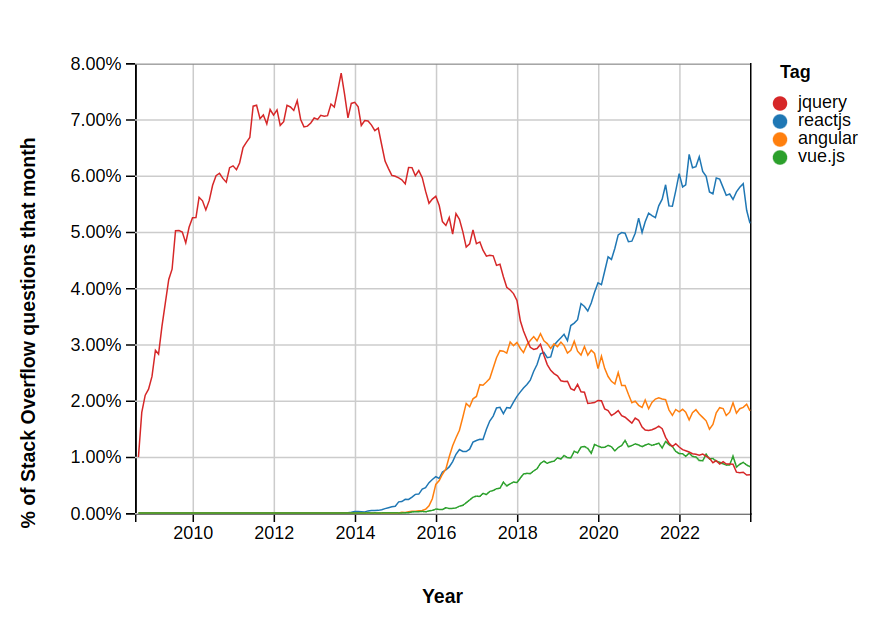
\includegraphics[width=0.9\linewidth]{figures/so-trends.png}
    \caption{Stack Overflow Trends JavaScript Frameworks (14/11/2023) (\cite{noauthor_stack_nodate})}
    \label{fig:so-trends}
\end{figure}

\begin{figure}
    \centering
    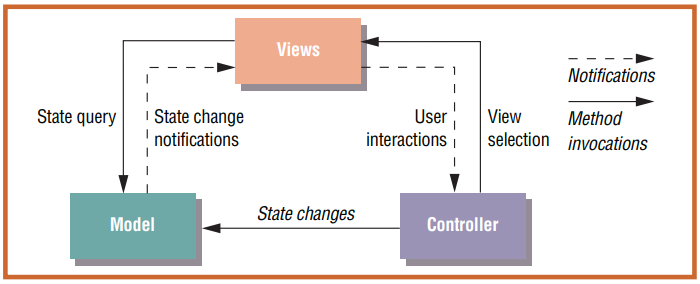
\includegraphics[width=0.9\linewidth]{figures/MVC.png}
    \caption{Model View Controller Model (\cite{curry_flexible_2008})}
    \label{fig:mvc-model}
\end{figure}

\clearpage

\subsection{React} 
\label{litrev:react}

The React.js framework was originally built by software engineers at Facebook with the intention of developing a JavaScript library for building user interfaces. React's main focus is to enable developers to "combine a number of short independent code fragments into a complex UI interface" (\cite{xu_benchmark_nodate}). React works similarly to the MVC (Model View Controller) model \see{fig:mvc-model}; it simply acts as the 'View' part of the model where it interacts with and utilises the VDOM (Virtual Document Object Model). When a state or props change occurs for a component, React compares the newly returned VDOM component with the previously rendered DOM component. If these components are not equal, the entire DOM is re-rendered (\cite{mariano_benchmarking_nodate}). 

\subsection{Next.js}
\label{litrev:next}

Next.js is a framework built on the original React.js framework and has recently become the new default for new React projects. It natively incorporates multiple production-ready such as server-side rendering. This feature, in particular, is one key improvement Next.js introduces whereby JavaScript modules are dynamically loaded on the server, drastically decreasing the client-side loading times (\cite{dinku_reactjs_2022}). Despite these improvements to React, introducing features such as server-side rendering can reduce the framework's compatibility with libraries such as Leaflet for OpenStreetMap which is pivotal to this project.

\subsection{Vue}
\label{litrev:vue}

In contrast to React, Vue was released in 2014, and instead of being built from the MVC model, it uniquely provides MVVM (Model View View-Model) data binding and a composable component system (\cite{xu_benchmark_nodate}). The MVVM data binding is two-way, where the component is divided into a model and a view; once the binding is created, the binding will be synchronised with the data (\cite{li_research_2021}). This enables Vue to have a similar state management system to React whereby the DOM will be re-rendered when the state of a component changes.

\begin{figure}
    \centering
    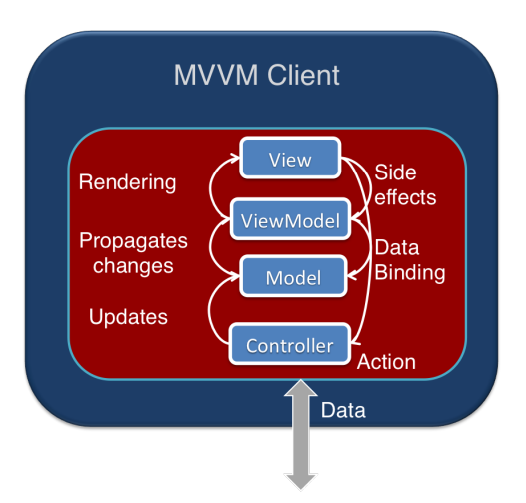
\includegraphics[width=0.5\linewidth]{figures/MVVM.png}
    \caption{Model View View-Model Model (\cite{zaris_-depth_nodate})}
    \label{fig:mvvm}
\end{figure}

\subsection{Angular}
\label{litrev:angular}
Angular has two separate versions, AngularJS (2010) and Angular2+ (2016); these are similarly both referred to as AngularJS; however, Angular2+ is the latest, maintained version based on Typescript, whereas AngularJS is built with JavaScript and is no longer actively maintained. Angular2+ is discussed within this review and will be referred to as Angular from now onwards.

Angular interacts with the DOM differently to React and Vue as Angular does not utilise the VDOM, instead handling only direct DOM manipulations (\cite{levlin_dom_2020}), but is still based on the MVC model \see{fig:mvc-model}. Angular interacts most similarly to JQuery out of all the modern frameworks. It implements create functions, such as \codeword{createCustomElement()}, which can be used to covert existing components into a class to be displayed on the DOM (\cite{levlin_dom_2020}). These classes contain decorators, which not only provide metadata but are also responsible for updating the component. Updates made to components via the decorator will update the existing DOM without the need to update a VDOM and compare it with the DOM (as done in React and Vue).

\section{Go (Programming Language)}
\label{litrev:golang}

Go, sometimes referred to as Golang, was developed by Google in 2007 and "arose through experience building large-scale distributed systems, working in a large codebase shared by thousands" (\cite{cox_go_2022}). Golang was built during a time when multi-core systems were becoming more and more common. Software Engineers at Google at the time found that the whole industry struggled to write efficient systems for multicore systems, and Go was their solution to the problem. Go has become increasingly popular over recent years \see{fig:gosograph}, primarily because the entire industry now faces those original issues highlighted by Google in 2007 when they were developing Go (\cite{cox_go_2022}).

Concurrency is one of Go's headline features. The language splits its concurrency model into two fundamental elements: Goroutines (lightweight threads) and Channels, which enable multiple Goroutines to communicate and synchronise execution (\cite{meyerson_go_2014}). Go follows the fork-join concurrency model; fork refers to how, at any point, it can split a child branch of execution which runs concurrently alongside the parent branch (\cite{cox-buday_concurrency_2017}). Once the child process has finished execution, it will rejoin the parent at the join \see{fig:forkjoin}.

\begin{figure}
    \centering
    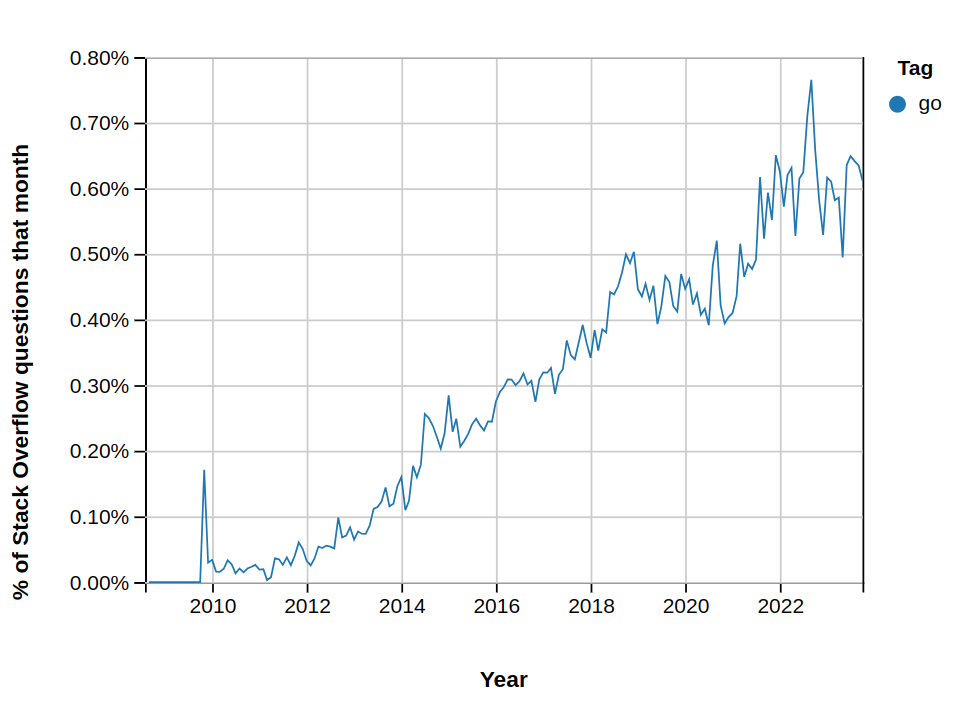
\includegraphics[width=0.8\linewidth]{figures/go-so-graph.png}
    \caption{Stack Overflow Trends Go (14/11/2023) (\cite{noauthor_stack_nodate-1})}
    \label{fig:gosograph}
\end{figure}

\begin{figure}
    \centering
    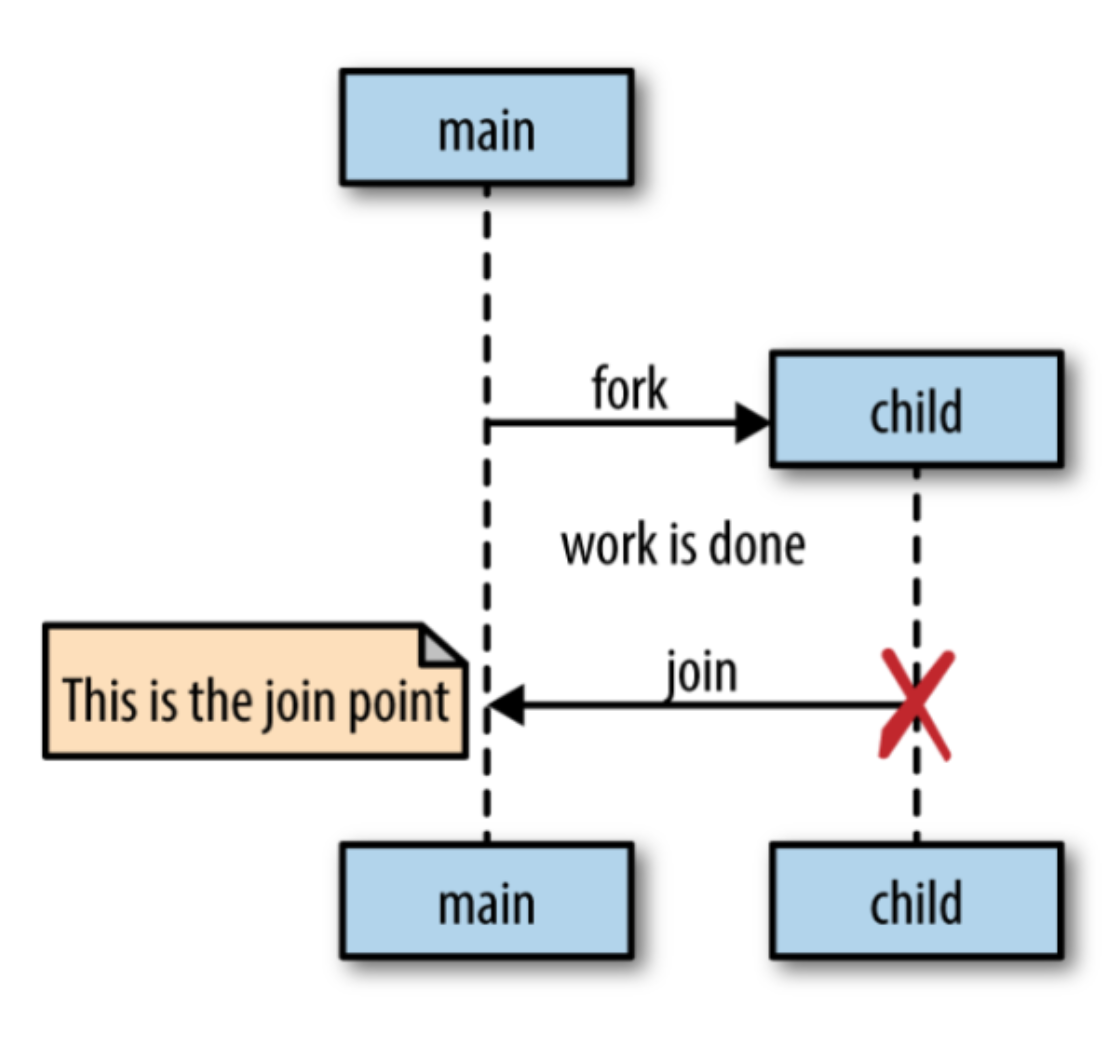
\includegraphics[width=0.5\linewidth]{figures/fork-join.png}
    \caption{Fork-Join Model (\cite{cox-buday_concurrency_2017})}
    \label{fig:forkjoin}
\end{figure}

\section{Competing Products}
\label{litrev:competingproducts}

There are many different route planners available with a range of different features, some common between applications and others specific to one. Applications like Plotaroute.com (\cite{noauthor_free_nodate}), Komoot (\cite{noauthor_komoot_nodate}) and Google Maps (\cite{noauthor_google_nodate}) have some commonalities, however serve slightly different purposes \see{fig:solutionsandfeatures}.

\begin{table}[h!]
    \centering
    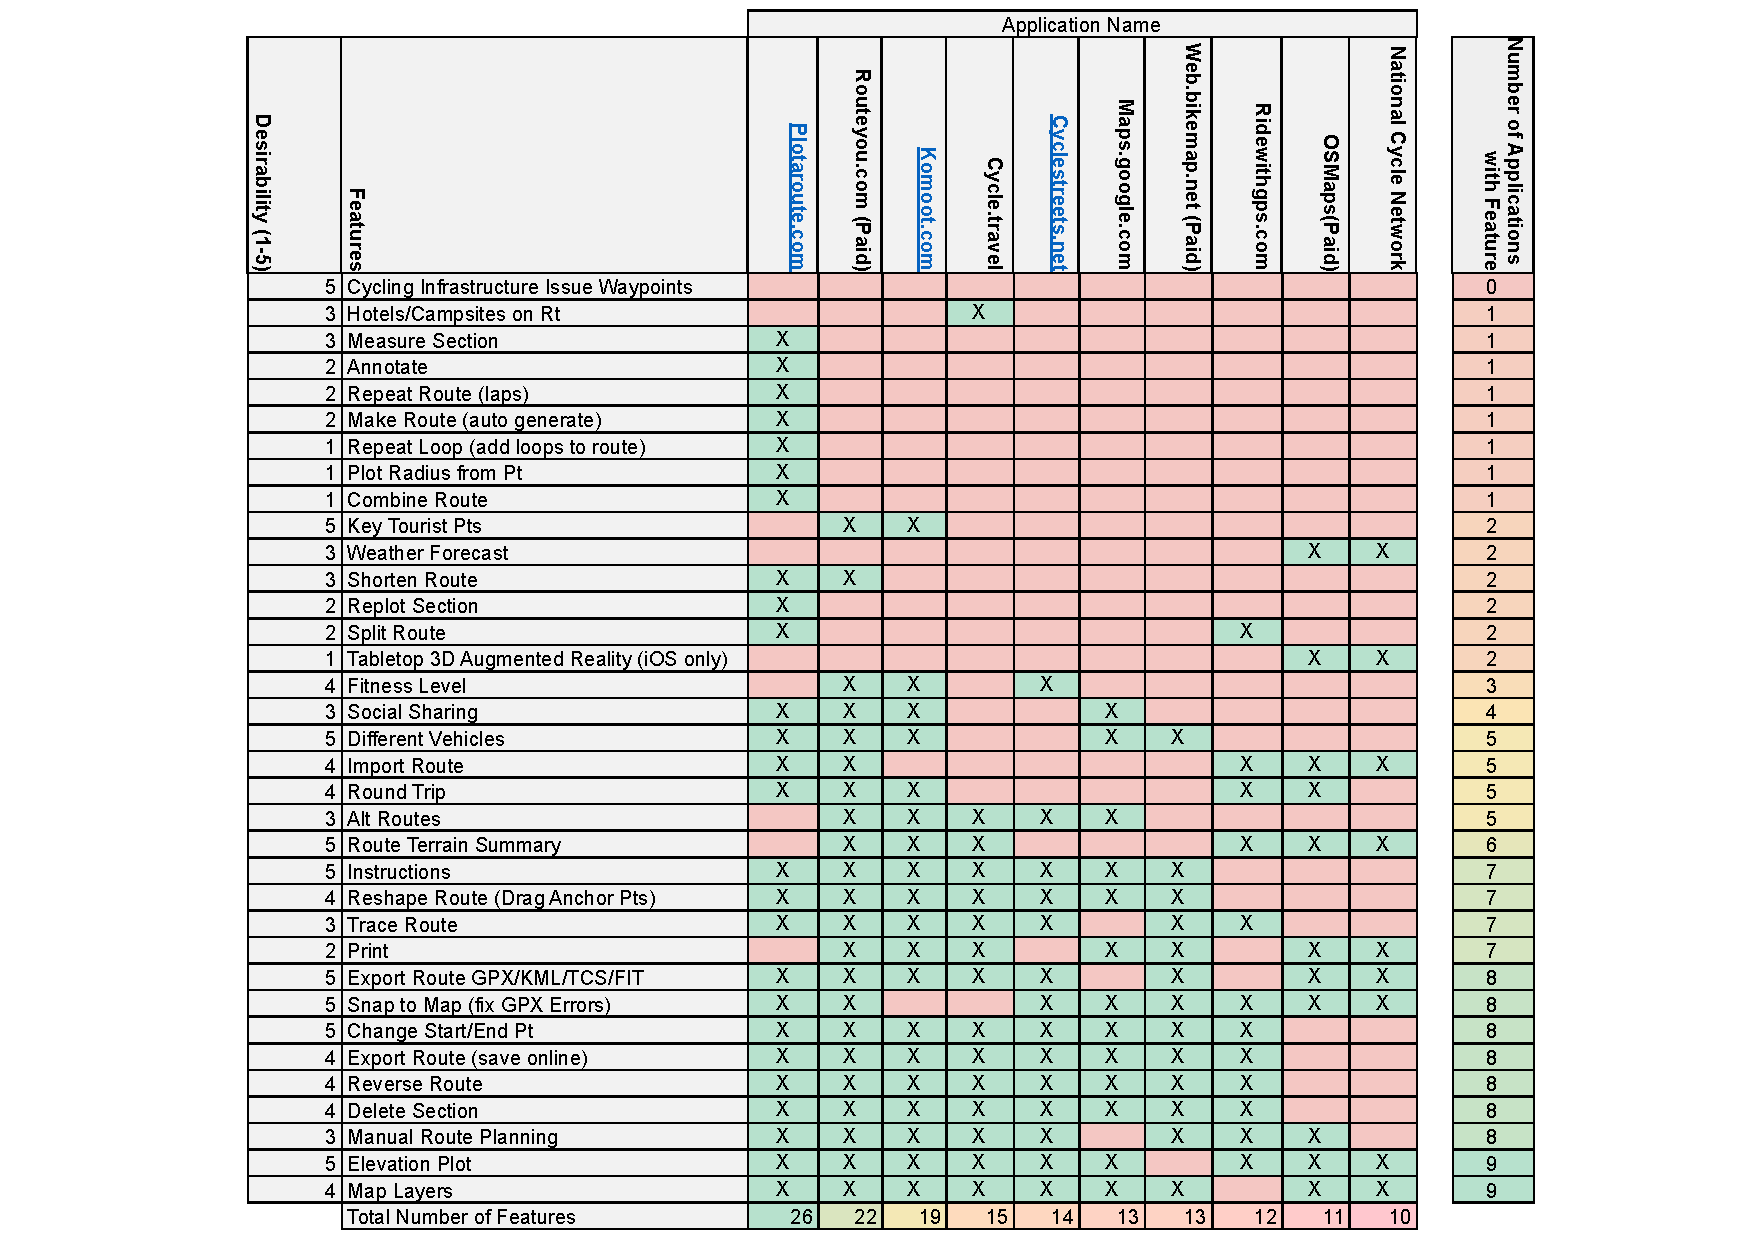
\includegraphics[width=1\linewidth]{figures/current_apps.pdf}
    \caption{Table of current solutions and their included features}
    \label{fig:solutionsandfeatures}
\end{table}

\subsection{Plotaroute.com}
\label{litrev:plotaroute}
Plotaroute.com (\cite{noauthor_free_nodate}), now referred to as Plotaroute, contains a wide range of features, including nearly all features highlighted in Figure 2.1 \see{fig:solutionsandfeatures}. The main shortfall of Plotaroute was identified as its UI (User Interface) rather than the features included. The UI of Plotaroute is very cluttered due to the number of features present in the application \see{fig:plotarouteui}. Unless the user is an expert and has used the application before, it is initially confusing what each part of the application does. Due to this, at first glace, it's unclear what type of route planner Plotaroute is, which will fundamentally affect a user's initial decision on whether or not to use the application.

\subsection{Komoot}
\label{litrev:komoot}
Komoot (\cite{noauthor_komoot_nodate}) offers a simpler-looking yet feature-rich application for planning and discovering routes \see{fig:komootui}. The application has a key focus on community, whereby a user doesn't necessarily need to plan a route, they can simply discover a route or even share a route of their own. This functionality allows the user to require minimal effort when planning location-specific rides, however doesn't offer discovery of longer routes, for example, Land's End to John O'Groats. When compared to Plotaroute, Komoot is clearly more user-friendly without sacrificing the core features needed by users. One primary setback with Komoot, however, is that some functionality for route planning is part of a paid-for service, therefore locking certain user bases out of some key desirable functionality.

\subsection{Google Maps}
\label{litrev:gmaps}

Google Maps (\cite{noauthor_google_nodate}) further reduces the specific functionality and offers a very simple, multi-functional route planning and location finding application \see{fig:gmapsui}. Google Maps is likely the most user-friendly out of all the applications, simply due to its simplicity and consistency across other Google applications (\cite{noauthor_material_nodate}). With this simplicity, however, most cycling-specific functionality is not present; the only option the user has when calculating a route is what the Google routing algorithm calculates with potentially a few alternate routes. Therefore, limiting how much the user can customise their route.

\begin{figure}[h!]
    \centering
    % 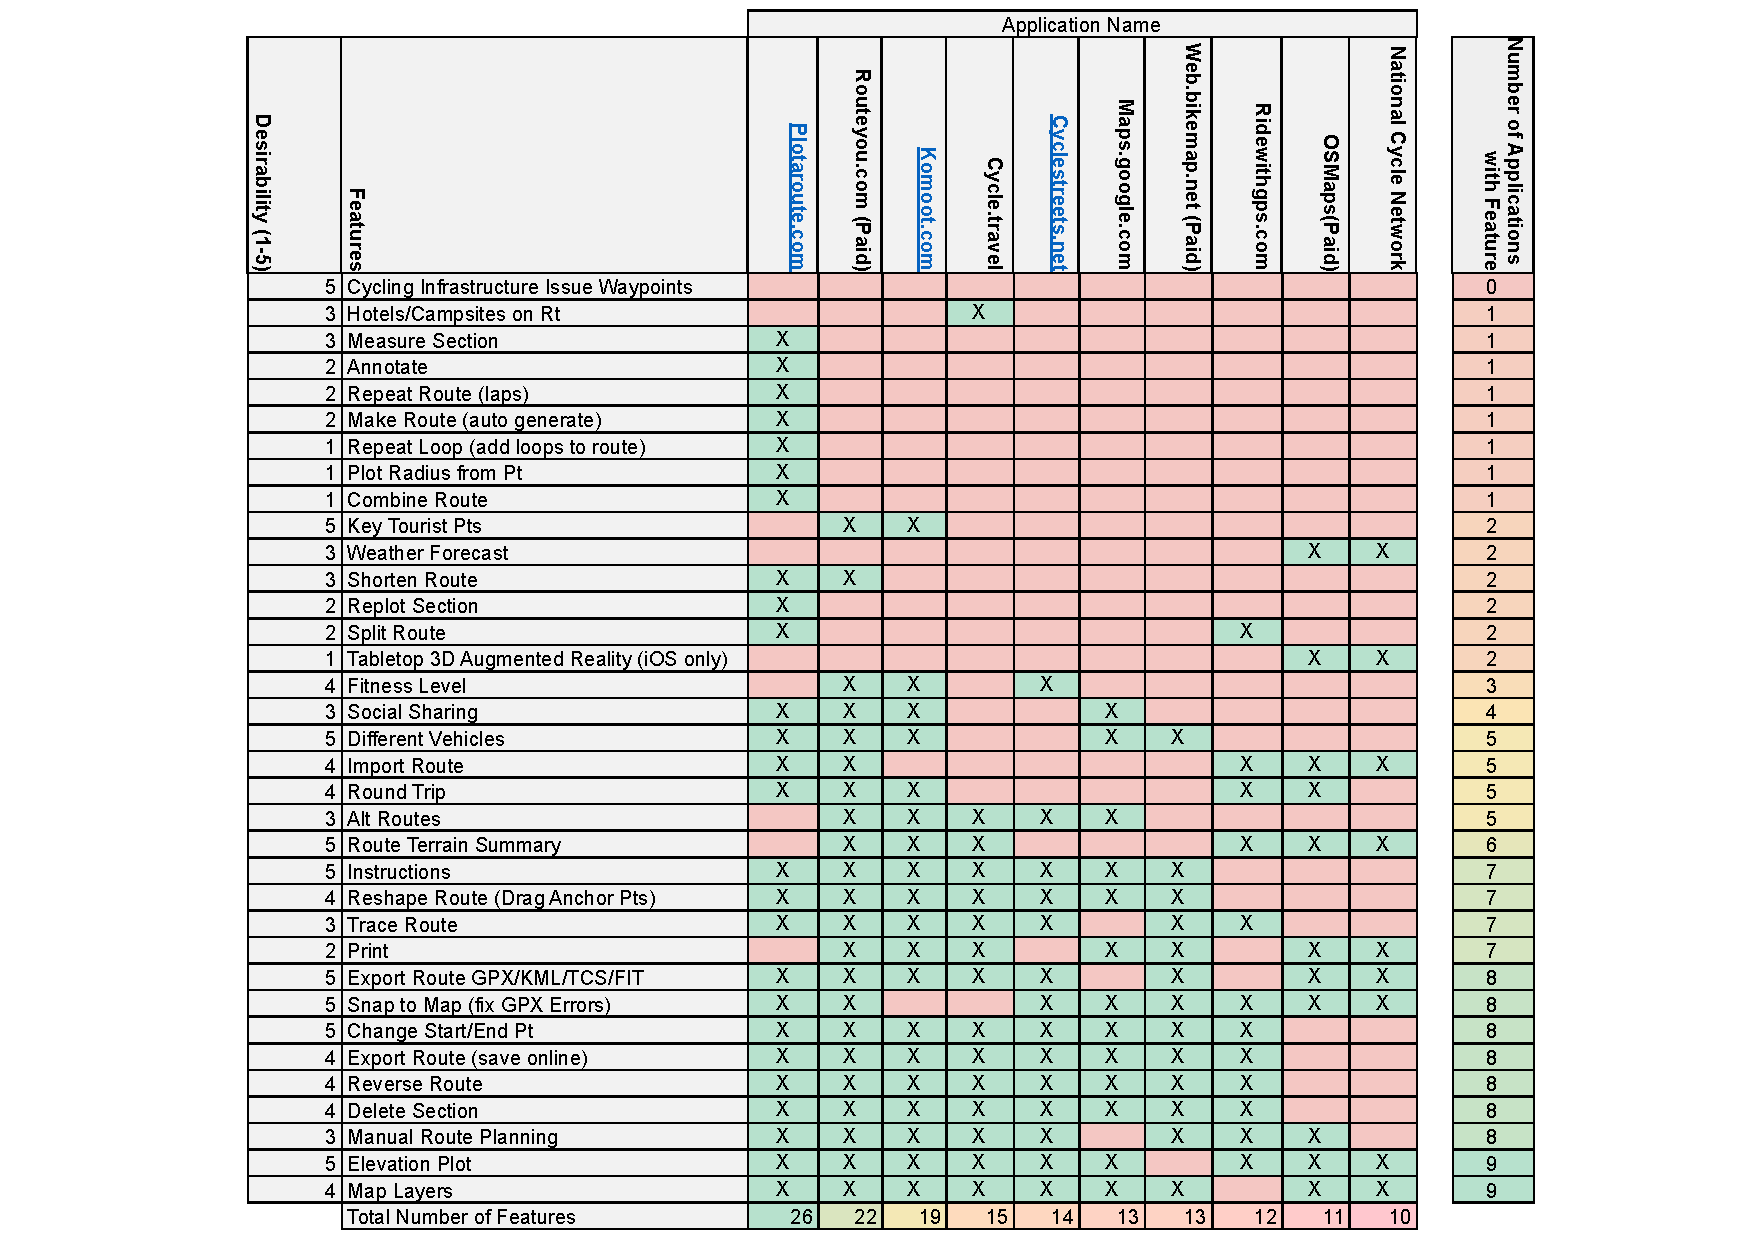
\includegraphics[width=1\linewidth]{figures/current_apps.pdf}
    \caption{Features in priority order based on user feedback}
    \label{fig:features}
\end{figure}

\section{Risk Factors in Route Planning}
Risk-based cycling route planning requires extensive knowledge of the impact of cycling and transportation infrastructure currently in place. It is also critical to understand how other external factors impact the risk of a route on an ever-changing basis. Within this section, a range of risk factors were explored to understand how multiple risk factors can be implemented into route planning algorithms.

\subsection{Cycling Infrastructure}
\label{litrev:cyclinginfrastructure}
The cycling infrastructure along a route must be understood because it is common for cyclists to share the same infrastructure as motorised vehicles. However, a cyclist has no physical protection if a crash occurs (\cite{reynolds_impact_2009}). There is often purpose-built infrastructure for cyclists, whether bike lanes alongside shared roads or off-road bike paths and this segregated infrastructure can help improve the safety of a route for a cyclist. Furthermore, Hong states how investing in effective cycling infrastructure "mitigates the negative effects of poor weather conditions" (\cite{hong_can_2020}), which further demonstrates that good, known infrastructure is key to improving the physical and perceived safety of a route in a range of different weather conditions. 

Furthermore, crowd-sourced data from route planners, cyclists and fitness applications such as Strava Routes (\cite{noauthor_strava_nodate}) have been key in developing new infrastructure. Boettge states how the most accurate assessment of a cycle network would come directly from the cyclists who use the network (\cite{boettge_assessing_2017}). Cyclists who use the network are the most familiar with the quality of each route and how traffic conditions improve the safety of the route. Utilising the GPS information from route planners and fitness tracking applications alongside direct input from cyclists can help build new routes and improve pre-existing routes, therefore preventing injuries and high-risk situations by modifying transportation infrastructure (\cite{reynolds_impact_2009}).

Areas with little to no cycling infrastructure, such as busy roads and roundabouts, force cyclists to have a heightened attentiveness that other road users don't have to consider due to not only the physical danger but the cyclists' perceived danger (\cite{doorley_analysis_2015}). These risks should be considered within route planning to decrease the number of 'risk' areas along a cyclist's route whilst also giving local areas the incentive to make infrastructure modifications to decrease the number of 'high-risk' points. Therefore, in the long-term, it will mitigate the need for constant action by cyclists to ensure their safety, which will, in turn, influence individuals' decisions to cycle (\cite{reynolds_impact_2009}).

Hull and O'Holleran also demonstrate how cities with a high reputation among cyclists also have safer roads and more attractive infrastructure. The Netherlands scored relatively equally amongst all categories, in comparison to cities with less of a reputation and, therefore, a lower standard of cycling infrastructure \see{fig:bicycleinfrastructurescorestable} \see{fig:bicycleinfrastructurescores} (\cite{hull_bicycle_2014}). This supports how Reynolds et al. further illustrate how investing in cycling infrastructure will greatly incentivise individuals to cycle due to the decreased risk. 

\begin{figure}
    \centering
    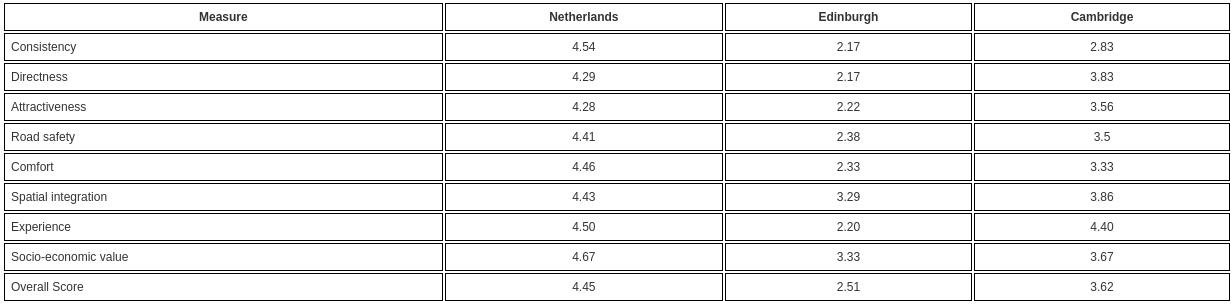
\includegraphics[width=400px, keepaspectratio]{figures/bicycle_infrastructure_score_table.jpg}
    \caption{Comparison of the bicycle infrastructure scores (\cite{hull_bicycle_2014}).}
    \label{fig:bicycleinfrastructurescorestable}
\end{figure}

\begin{figure}
    \centering
    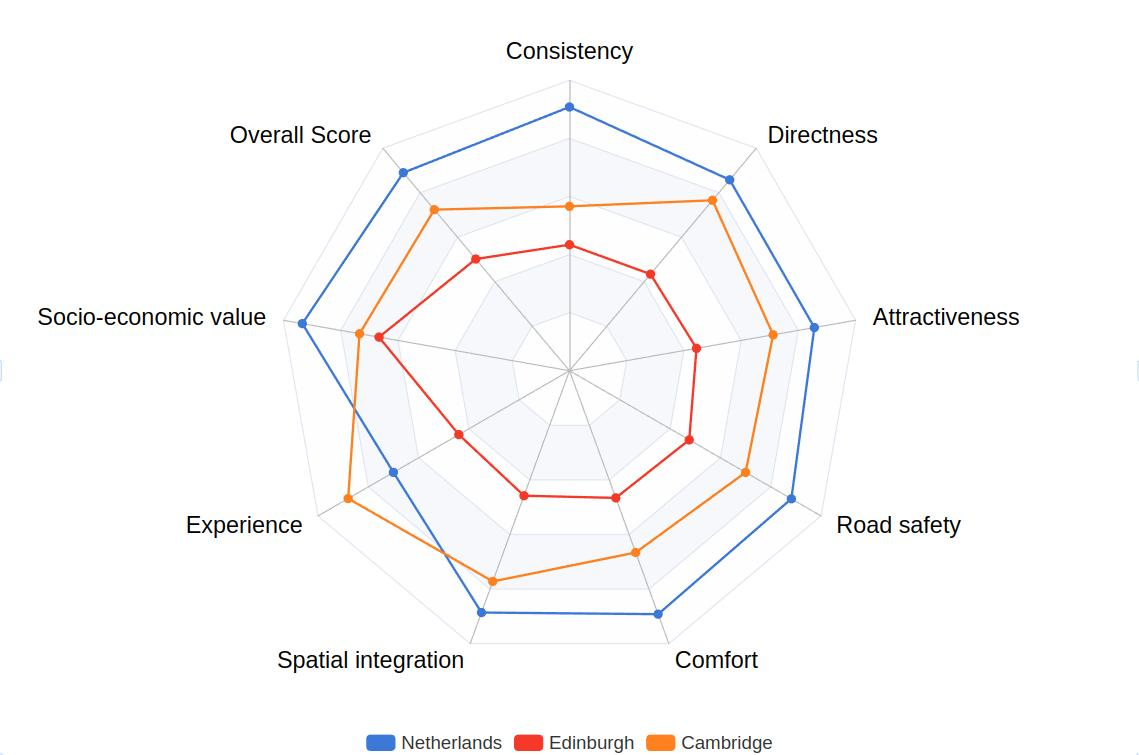
\includegraphics{figures/bicycle_infrastructure_scores.jpg}
    \caption{Spider web diagram comparing the Bicycle Infrastructure Scores (\cite{hull_bicycle_2014}).}
    \label{fig:bicycleinfrastructurescores}
\end{figure}

\subsection{Weather Conditions}
\label{litrev:weatherconditions}
Weather conditions will also have a pivotal effect on how a route planner will calculate the safest route for a cyclist. Following on from Cycling Infrastructure \see{litrev:cyclinginfrastructure}, it is demonstrated how a lack of good infrastructure goes hand-in-hand in creating an unsafe route alongside the weather. To ensure the safety of cyclists, all routes and road surfaces must be maintained to withstand different weather conditions (\cite{shoman_evaluation_2023}).

The weather also impacts a cyclist's likelihood to ride; Flynn states that cyclists "were nearly twice as likely to commute by bicycle when there was no morning precipitation" (\cite{flynn_weather_2012}). It is clear that even minor changes in the weather can drastically affect a cyclist's decision to ride, further demonstrating how vital the perceived safety of cycling is in deciding whether to ride. 

Contrasting this, Hull and O'Holleran state that the main environmental barriers included too much traffic, too many hills, no bike lanes/trails, no safe place to cycle and badly maintained streets (\cite{hull_bicycle_2014}). Therefore suggests that the weather should have a minimal impact on a cyclist's decision to ride if the infrastructure is sufficient. Despite the findings of Hull and O'Holleran, it seems to be a common finding that the perceived safety of cycling, both in regard to the changing weather conditions and cycling infrastructure, is the primary factor in choosing cycling over an alternative method of transport. Miranda-Moreno and Nosal have shown how when infrastructure is implemented, there is generally an increase in total bicycle usage and diversion of cyclist flows away from roads to purpose-built infrastructure even in less ideal weather conditions (\cite{miranda-moreno_weather_2011}).

\section{Conclusion}
\label{litrev:conclusion}

To conclude, route planning with different customisable preferences has been implemented by a range of different existing organisations; however, focusing on a risk-based routing approach has not been addressed by these existing solutions. Utilising pre-existing routing algorithms such as Open Route Service (\cite{noauthor_openrouteservice_nodate}) or Open Source Routing Machine (\cite{noauthor_project_nodate}) and integrating custom, weather and infrastructure data alongside the usual user-preferences has not been implemented within existing solutions. Therefore, this enables a unique system to be developed whereby crowd-sourced infrastructure data alongside weather data provided by OpenWeatherMap (\cite{noauthor_urrent_nodate}) combined form a risk index utilised in a customised routing algorithm.

Furthermore, in order to develop this system, React.js was chosen to develop the front end and Go for the back end. Next.js was initially considered for the front-end. However, it was later found that Next's server-side rendering was not supported by Leaflet; used for Mapping with OpenCycleMap; (\cite{noauthor_leaflet_nodate};\cite{noauthor_opencyclemaporg_nodate}) due to it requiring direct interaction with the DOM. Go with the Gin Web Framework (\cite{noauthor_gin_nodate}) was chosen to develop the API and back-end due to its increased performance benefits over alternative languages such as Node.js with Express.js.